  \begin{figure}[H]
%\begin{wrapfigure}[10]{L}{0.45\textwidth}
\vspace{-15pt}
%  \begin{center}
  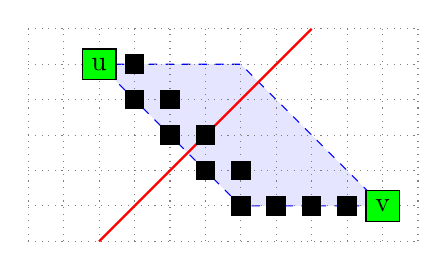
\begin{tikzpicture}[scale=0.45]
    \draw[blue, dashed, fill=blue!10] (2,5) -- (6,5) -- (10,1) -- (6,1) -- cycle; 
    \draw[color=gray, style=dotted] (0,0) 
      grid[xstep=1cm, ystep=1cm] (11cm,6cm);
  	\node at (2,5) [draw,fill=green] {u};
  	\node at (10,1) [draw,fill=green] {v};
	\draw[red,thick] (2,0) -- (8,6); 
    \node at (3,5) [draw, fill=black] {};
    \node at (3,4) [draw, fill=black] {};
    \node at (4,4) [draw, fill=black] {};
    \node at (4,3) [draw, fill=black] {};
    \node at (5,3) [draw, fill=black] {};
    \node at (5,2) [draw, fill=black] {};
    \node at (6,2) [draw, fill=black] {};
    \node at (6,1) [draw, fill=black] {};
    \node at (7,1) [draw, fill=black] {};
    \node at (8,1) [draw, fill=black] {};
    \node at (9,1) [draw, fill=black] {};
  \end{tikzpicture}
  \caption{Every line parallel to $l$ with $u$ and $v$ on different sides must contain one of the vertices marked with black squares.}
  \label{gaphull2}
%  \end{center}
  \end{figure}
%\end{wrapfigure}
